\documentclass[a4paper,twoside,11pt]{article}
\usepackage{a4wide,algo,graphicx,fancyhdr,amsmath,amssymb,amsthm,ifthen,path,todonotes}
\usepackage{subcaption, caption}
\usepackage[ruled, noline, algo2e, noend]{algorithm2e}
\usepackage{hyperref}
\usepackage{url}
\usepackage{color}
\urlstyle{rm}
\usepackage{tikz}
\usepackage{xifthen}
\usepackage{listings}
\usepackage{pgfplots}
\usepackage{comment}
\usepackage{parskip}
\usepackage{tabularx, colortbl}
\usepackage{mathtools}
\usepackage{amsmath}
\usepackage{float}
%----------------------- Macros and Definitions --------------------------
\graphicspath{ {./img/} }

\setlength\headheight{10pt}
\addtolength\topmargin{-10pt}
\addtolength\footskip{20pt}

\newenvironment{myindentpar}[1]%
{\begin{list}{}%
	{\setlength{\leftmargin}{#1}}%
	\item[]%
}
 {\end{list}}

\fancypagestyle{plain}{
\fancyhf{}
\fancyfoot[LO,RE]{\sffamily\bfseries Eindhoven University of Technology}
\fancyfoot[RO,LE]{\sffamily\bfseries\thepage}
\renewcommand{\headrulewidth}{0pt}
\renewcommand{\footrulewidth}{0pt}
}

\newcommand{\List}{\mathcal{L}}
\newcommand{\T}{\mathcal{T}}
\newcommand{\G}{\mathcal{G}}
\newcommand{\s}{\mathcal{S}}

\newcommand{\opt}{\textsc{opt}}

\pagestyle{fancy}
\fancyhf{}
\fancyhead[LE]{\sffamily\bfseries }
\fancyhead[RO]{\sffamily\bfseries Project1 - Particles}
\fancyfoot[LO,RE]{\sffamily\bfseries 2IV15 Simulation in computer graphics - Eindhoven University of Technology}
\fancyfoot[RO,LE]{\sffamily\bfseries\thepage}

%-------------------------------- Title ----------------------------------

\title{\sffamily\bfseries
Project1 \\[1ex]
\large Particles
}

\author{
    Wouter Lok \\
    Student number: 0832518 \\
    \texttt{w.lok@student.tue.nl}
    \and
    Joris Reijrink \\
    Student number: 0847198 \\
    \texttt{j.reijrink@student.tue.nl}\\
}

\date{\today}

\setlength{\parindent}{24pt}

% Set \item separation length
%\newlength{\wideitemsep}
%\setlength{\wideitemsep}{1\itemsep}
%\addtolength{\wideitemsep}{-7pt}
%\let\olditem\item
%\renewcommand{\item}{\setlength{\itemsep}{\wideitemsep}\olditem}


%--------------------------------- Text ----------------------------------

\begin{document}

\maketitle
\newpage

\vspace{1cm}

\section{Introduction}
In this report, we describe the results of the implementation of a particle system with constraints. The system is able to solve and simulate forced applied to particles while taking into account the constrains of the particles. Forces and constraints are applied in a generalized structure such that new forces and constraints can be added easily.
\section{Forces}
The system implements two forces; \emph{gravity} and \emph{damped spring} force. The spring force is implemented according to a behaviour function $C(x_1, x_2, ..., x_n)$, which evaluates to zero if the desired state of the particle(s) is reached. Since gravity does not have a rest value, it not implemented using this function. Forces are implemented using an abstraction, such that the system can maintain a list of forces. Then for each time forces have to be applied, the system can easily over the force-list to apply the forces to the particles.\\
Gravity force is defined as $f_{grav} = mG$, where $m$ is the mass of a particle and $G$ is a gravitational constant. The damped spring force acts like a normal spring between two particles $p_1$ and $p_2$ with rest length $l$. The force applied by the spring on $p1$ is defined as $f_{p_1} = (k_s (|l| - r) + k_d \frac{i \dot l}{|l|}) * \frac{l}{|l|}$, where $l = x_{p_1} - x_{p_2}$ and $i = v_{p_1} - v_{p_2}$, $k_s$ is the stiffness of the spring and $k_d$ is a damping constant. 
\section{Constraints}

The constraints are implemented using a generic solver.
..
\\

Each constraint is implement using the \verb"Constraint" interface.
This interface requires a constraint to have the following functions:
\begin{itemize}
  \item GetC\\
  \emph{ This function contains the constraint }
  \item GetCdot\\
  \todo { wat hier? }
  \item GetDerivative\\
  \emph{ This function contains the partial derivative of the constraint  }
  \item GetTimeDerivative\\
  \emph{ This function contains the time derivative of the constraint }
\end{itemize}

All constraints are resolved using the
To resolve all constraint the
\noindent Calculate $J$, the jacobian matrix.\\
We loop through all constraints and add their GetDerivative() values to the appropriate places in the matrix.
The resulting matrix has the structure as shown in figure \todo { verwijzing }, where $C$ is a constraint and $x$ is a particle.
\todo{ image jacobian matrix }

Calculate $W$, inverse mass \\
Calculate $\dot{J}$, jacobian time derivative matrix\\
Calculate $\dot{q}$, velocity vector\\
Calculate $Q$, constraint force vector\\
Calculate $C$, constrain vector\\
Calculate $\dot{C}$, partial derivative of constraints vector\\
$k_s$ and $k_d$ are constants used for..\\
Solve $Ax = B$ where\\
\;\;  $A = J W J^{T}$\\
\;\;  $B = (-\dot{J} \dot{q}^{T} - J W Q^{T}) - (C k_s) - (\dot{C} k_d)$\\
We added the feedback term $- (C k_s) - (\dot{C} k_d)$ to prevent drifting in the constraint force calculation.
With the calculated $x$ matrix we can calculate the constraint forces matrix using the formula $x^{T} J$.
The forces of each particles are updated using this resulting constraint forces matrix.\\

\subsection{Rod}
Used for..\\
Impl\\

\subsection{CircularWire}
Used for..\\
Impl\\

\subsection{FixedLine}
Horizontal and vertical\\
Used for..\\
Impl\\

\subsection{FixedPoint}
Used for..\\
Impl\\

\section{Interaction}

Mouse interaction:\\
- Select particle\\
- Horizontal force\\

\section{Integration}
To be able to simulate the particles with more precision, we have implemented multiple integration schemes. This has been done, since the euler method is very unstable and can explode very fast. Therefore we have implemented the following integration schemes:
\begin{itemize}
  \item[-] Euler, convert current force to acceleration and apply acceleration to current velocity weighted by the current time-step. Then update the position by the new velocity again weighted by the current time step.
  \item[-] Mid-Point, firstly backup the positions and velocities of the current particles. Then for each particle, calculate a intermediate velocity using the euler method and calculate the midpoint position with half the current time step. Then take another euler step from the midpoint. Finally restore the original position of all the particles and update the positions by the new midpoint velocity weighted by the the time step.
  \item[-] Runge-Kutta 4-order, similar to midpoint, but forces and constraints are evaluated four times. After each evaluation, the position of all the particles are reset and updated according to the new velocities calculated during the previous force/constraint evaluation, weighted by a fraction of the timestep. The final velocity is calculated by $v_f = v_{t0} + \frac{v_{k_1}}{6} + \frac{v_{k_2}}{3} + \frac{v_{k_3}}{3} + \frac{v_{k_4}}{6}$, where $v_{k_x}$, is the velocity of the particles after the $xth$ evaluation. In the end, the positions of each particles is again updated by the final velocity weighted by the time step.
\end{itemize}
The difference of the integration schemes can be notices easily. As displayed below, the Runga Kutta method is more stable than euler. Furthermore, we noticed that for our configuration, that the midpoint integration method was a little more stable than euler. Euler method easily explodes at around time-step 0.03 with interaction, but midpoint also exploded quite easily with interaction with time-step 0.039 by using interaction. Runga kutta start exploding with lots of interaction when using time-step 0.069s.

\begin{figure}[!htbp]
  \begin{subfigure}[h]{\textwidth}
  \centering
    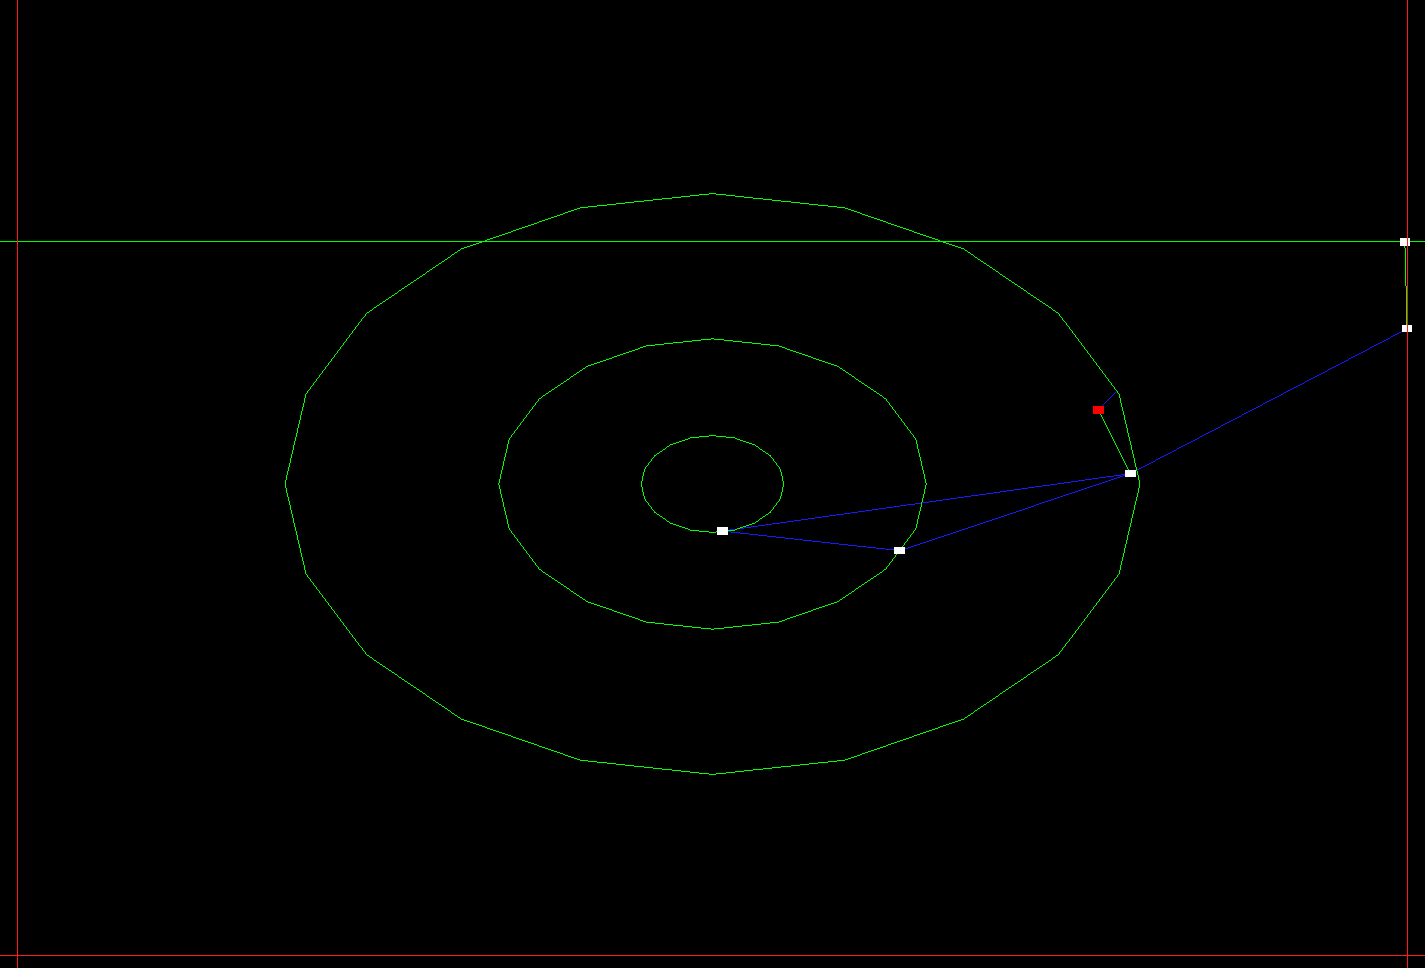
\includegraphics[width=0.4\textwidth]{euler1}
    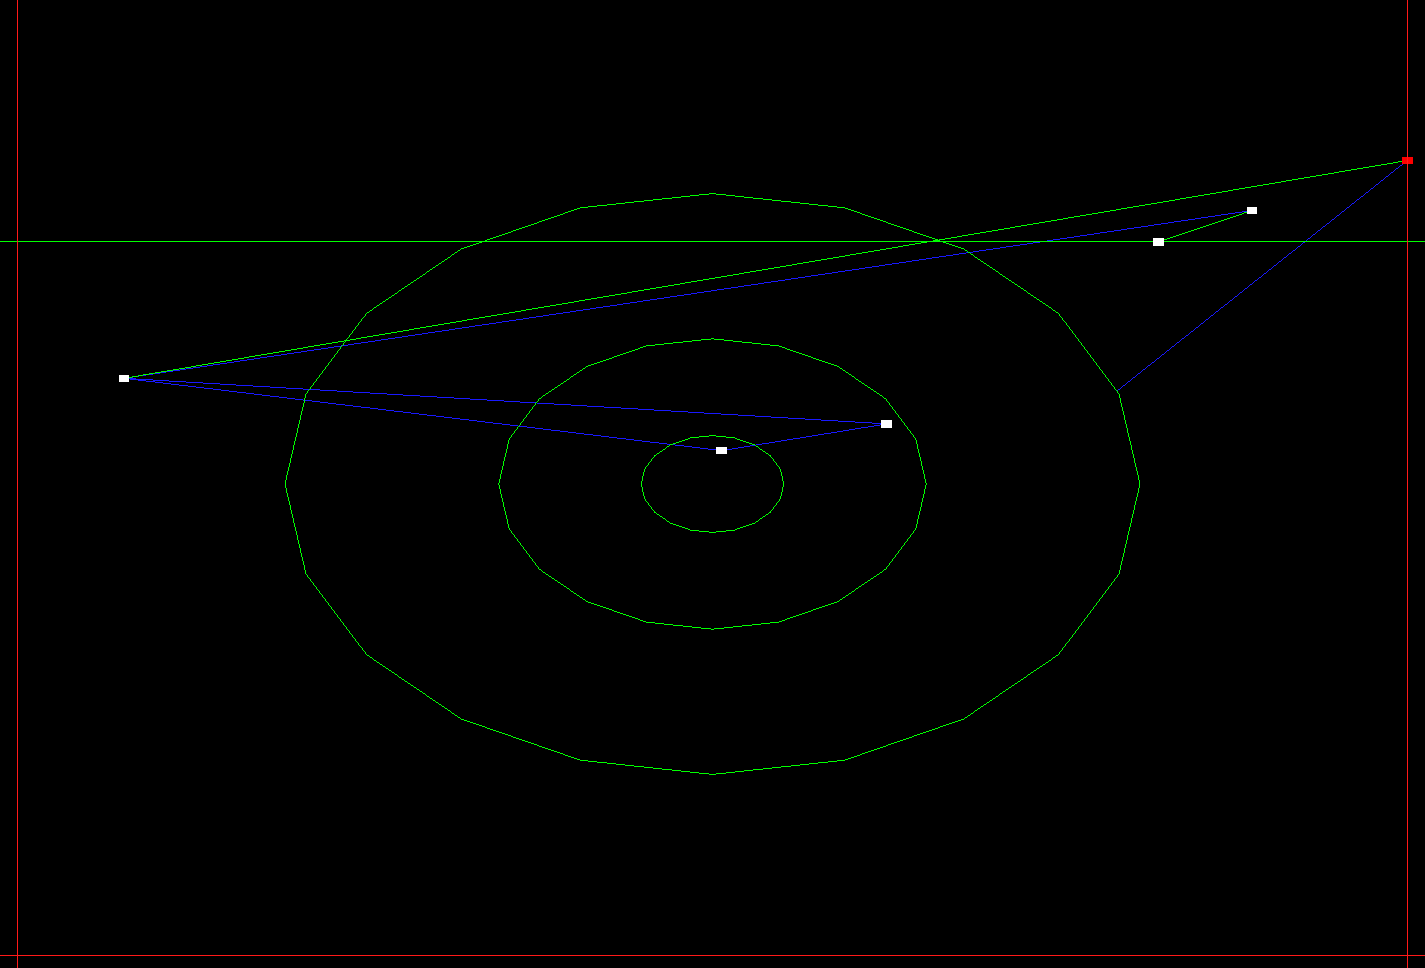
\includegraphics[width=0.4\textwidth]{euler2}
    \caption{Euler integration explodes after short time at time-step 0.04s}
    \label{fig:euler}
  \end{subfigure}
  \\
  \begin{subfigure}[h]{\textwidth}
  \centering
    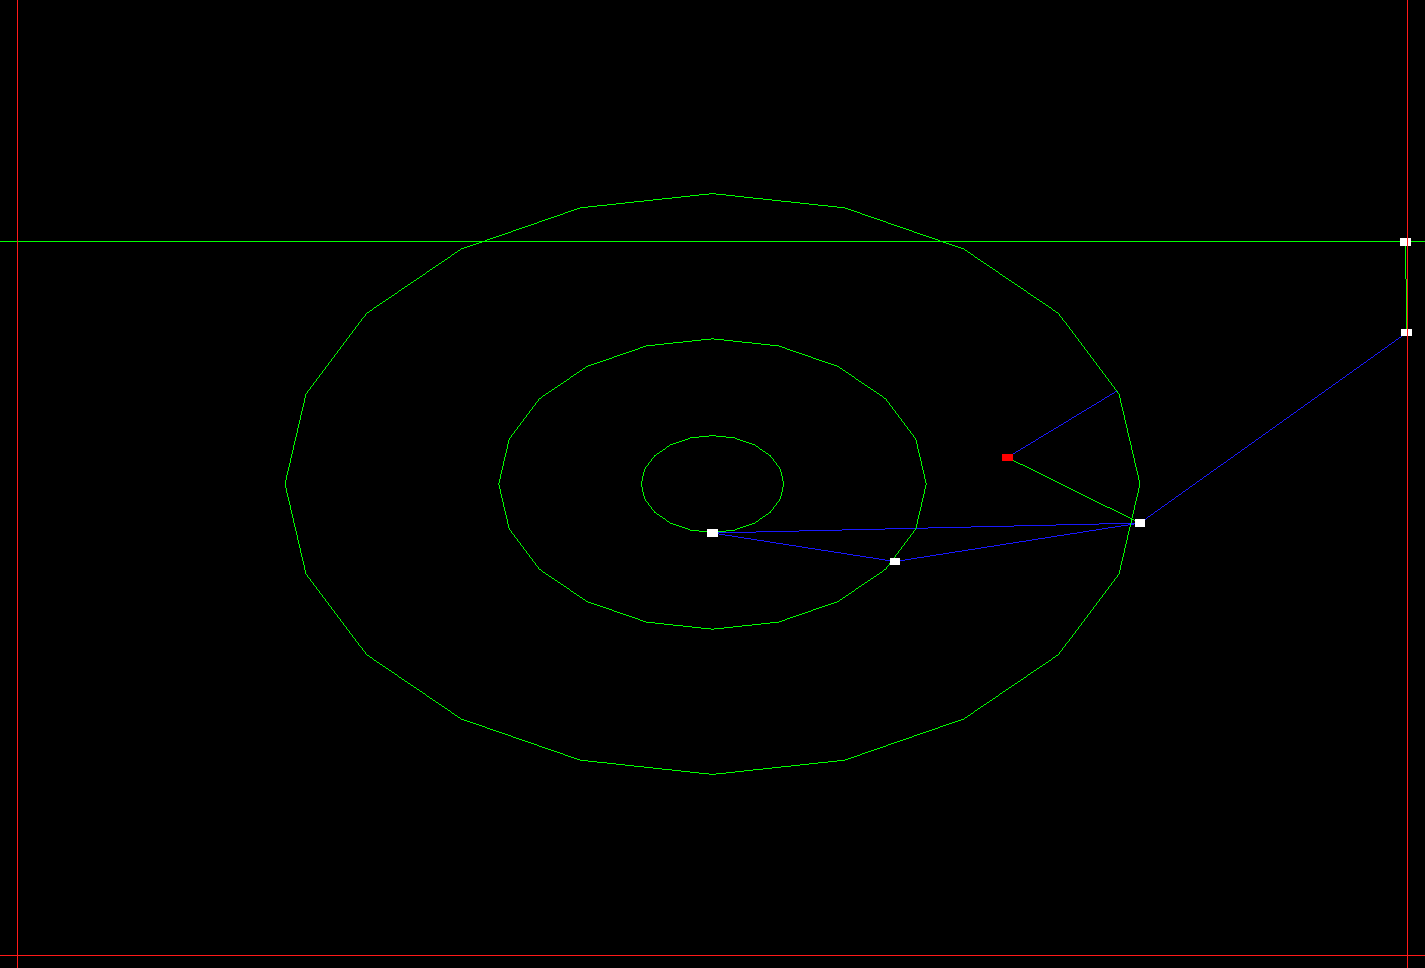
\includegraphics[width=0.4\textwidth]{runga1}
    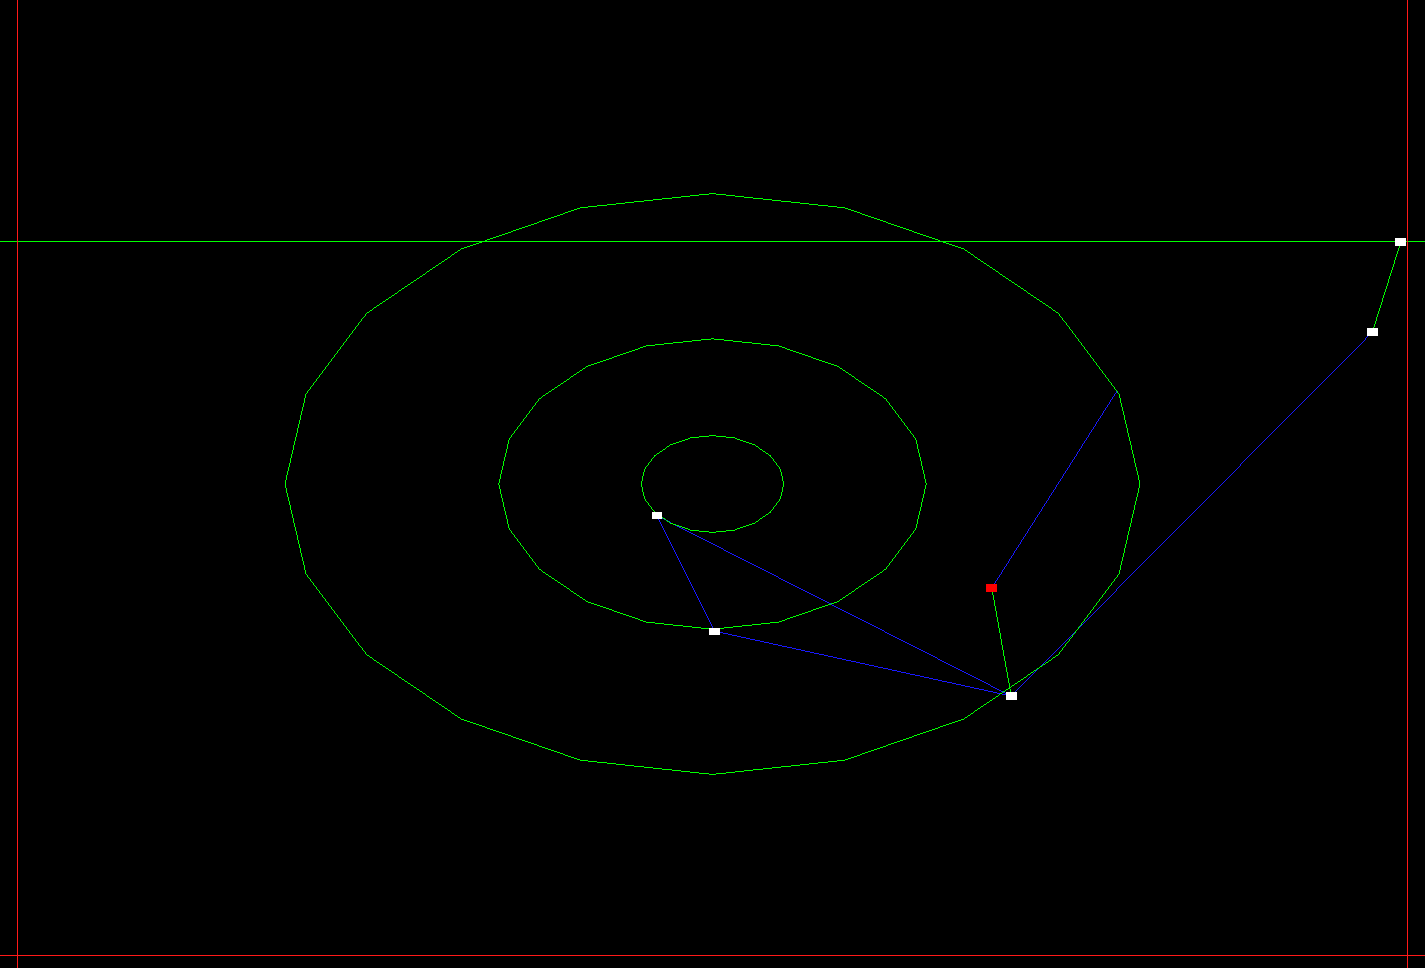
\includegraphics[width=0.4\textwidth]{runga2}
    \caption{Runga Kutta integration stays stable at time-step 0.04s}
    \label{fig:ruga}
  \end{subfigure}

  \caption{Comparison Euler and Runga Kutta integration scheme}
  \label{fig:integration}
\end{figure}

\section{Cloth}

\begin{figure}[h!]
\centering
\begin{minipage}[t]{.45\textwidth}
  \centering
  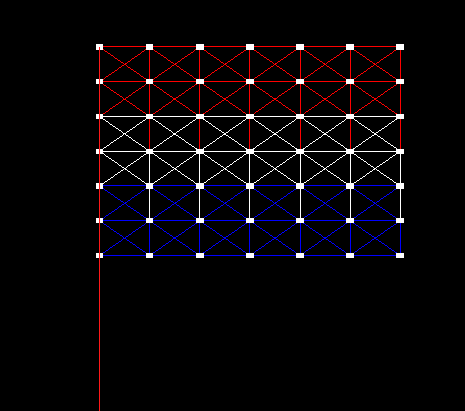
\includegraphics[width=7cm]{img/flag.png}
  \captionof{figure}{Start position of the cloth flag}
  \label{fig:flag}
\end{minipage}\hfill
\begin{minipage}[t]{.45\textwidth}
  \centering
  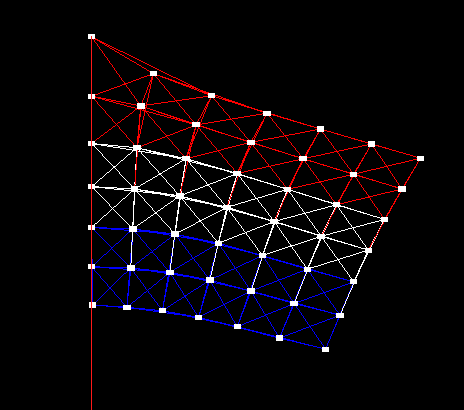
\includegraphics[width=7cm]{img/flag2.png}
  \captionof{figure}{Position after some iterations}
  \label{fig:flag2}
\end{minipage}
\end{figure}

\noindent The structure of the cloth contains of multiple spring forces.
First a grid of spring forces is created.
Then in each cell of the grid two cross springs are added, creating a cross in each cell.
Finally a spring of twice the length is added to each point of the grid, connecting two cells.
This structure will result in quite a realistic piece of cloth.
In figure ~\ref{fig:flag} and ~\ref{fig:flag2} a Dutch flag is modeled, the pole is a fixed object with a particle constrained in the left top using a Fixed constraint. Also all left particles are constraint using a vertical line constraint.
\section{Hair}
To simulate hair, angular springs are used. Our implementation of the angular spring is not directly based on a behaviour function, but instead combines the usage of damped springs and rod constraints such that a triplet of particles are pulled so that their subtending angle approaches some rest angle. In figure \ref{fig:Angular Spring}, the structure in which the springs and rods are configured is shown. \\
\begin{figure}[h]
    \centering
    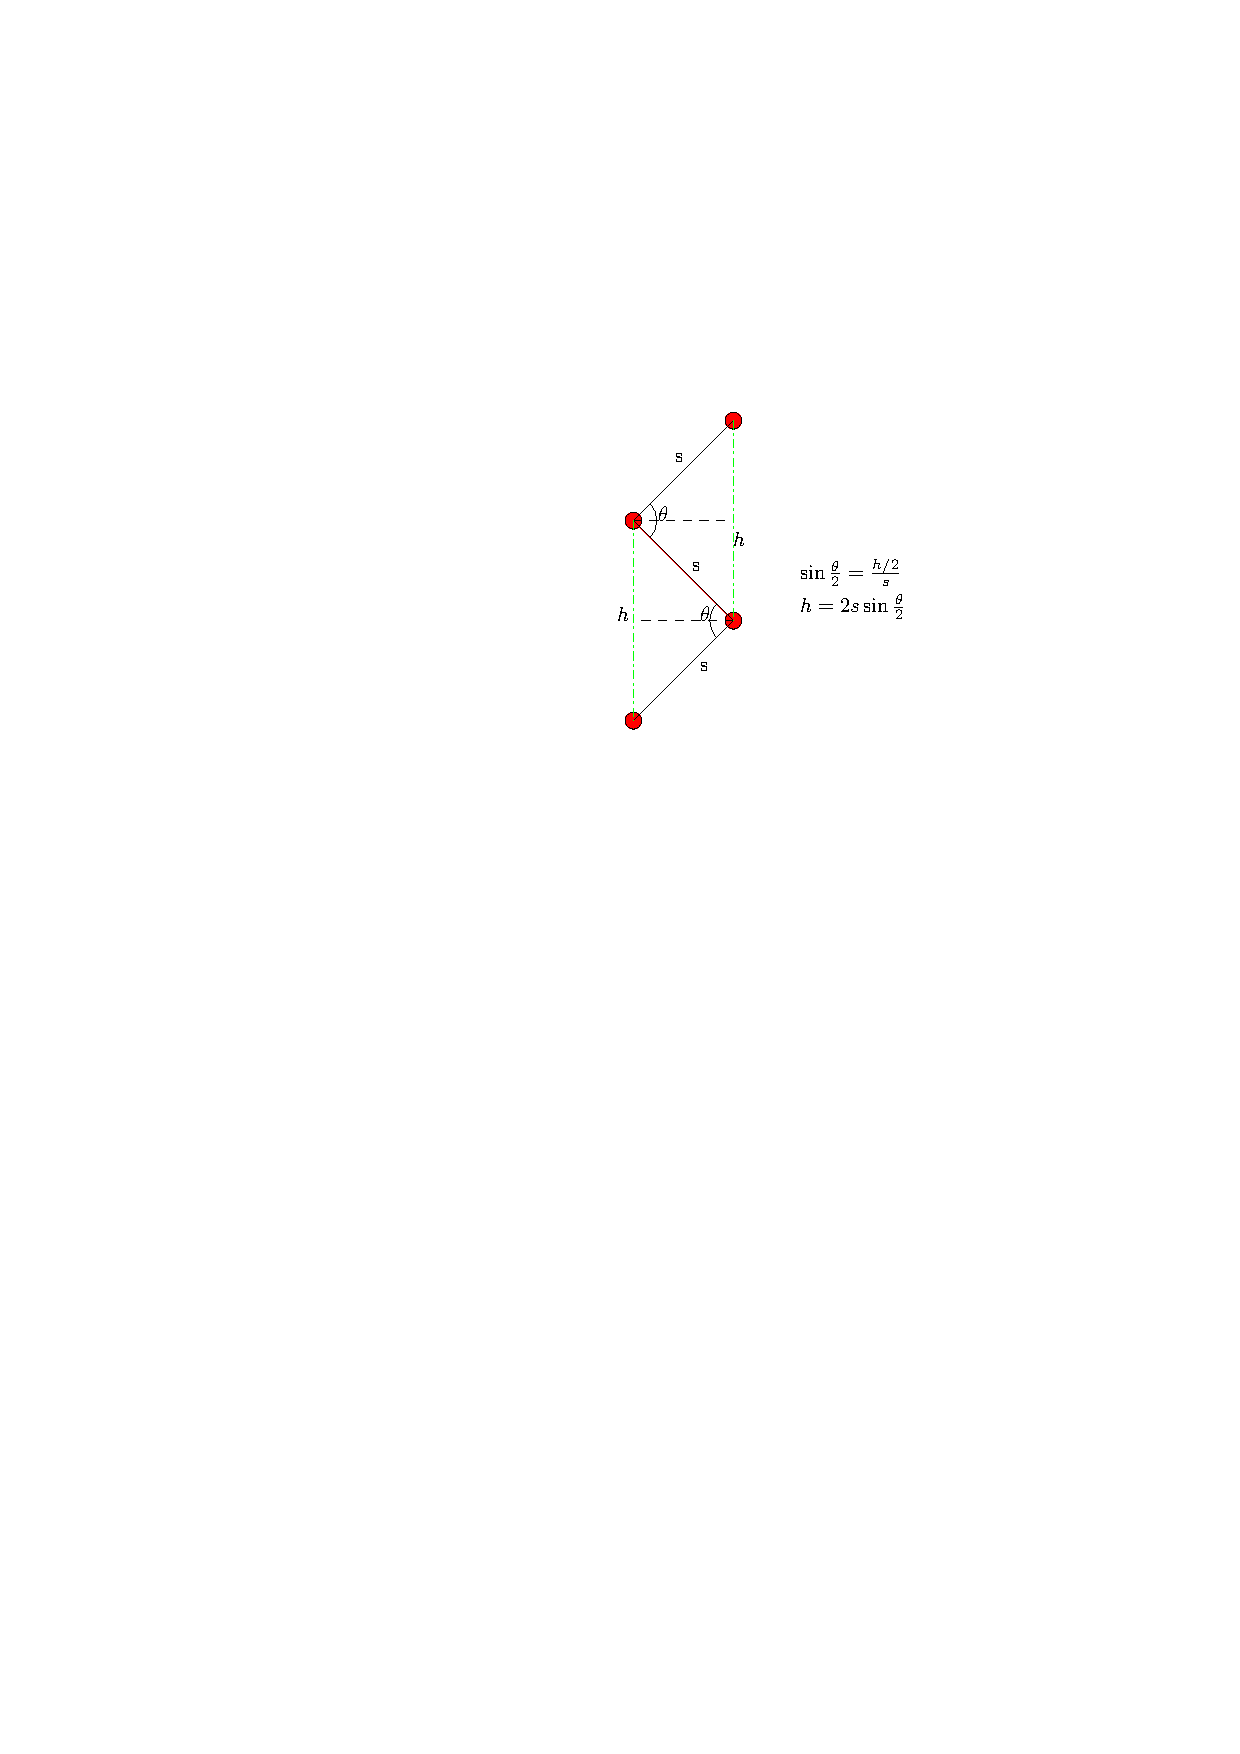
\includegraphics[width=0.4\textwidth]{hair}
    \caption{Representation angular spring}
    \label{fig:Angular Spring}
\end{figure}
The green dotted dashed lines in the figure are representing springs with rest length $h$ and the black solid lines are representing rod constraints of length $s$. The calculations to calculate the rest length is also given for some rest angle $\theta$. In this way, the rods will ensure that each hair segments is of constant length and the damped springs will pull or repel the first and the last particle until the rest angle is reached.\\
By using the last particle of the tripled as the first particle of a new triplet, it is possible to create a chain which can represent a string of hair.
\section{Collisions}

Collision detection:\\
- Fixed objects\\
- Paticles\\

\section{Results}
In the figures below some scenes are shown of the final result.

\begin{figure}[h!]
\centering
\begin{minipage}[t]{.40\textwidth}
  \centering
  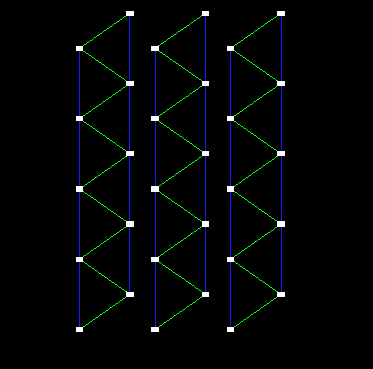
\includegraphics[height=5cm]{img/resulthair.png}
  \captionof{figure}{Start position of hair}
  \label{fig:hair}
\end{minipage}\hfill
\begin{minipage}[t]{.50\textwidth}
  \centering
  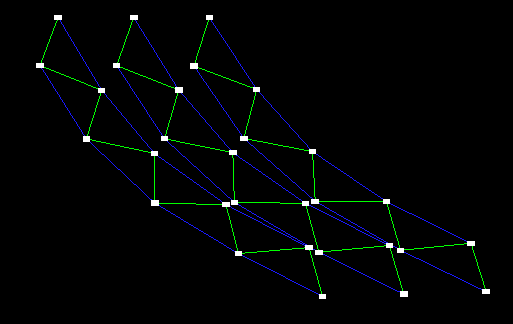
\includegraphics[height=5cm]{img/resulthair2.png}
  \captionof{figure}{Hair position after some iterations}
  \label{fig:hair2}
\end{minipage}
\end{figure}

\begin{figure}[h!]
\centering
\begin{minipage}[t]{.45\textwidth}
  \centering
  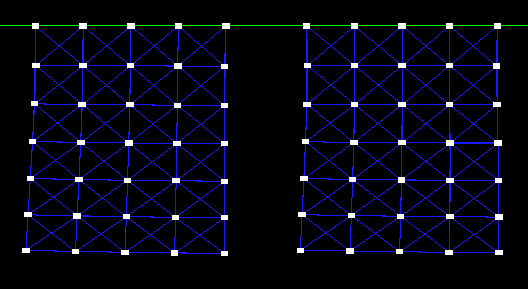
\includegraphics[height=4cm]{img/curtain.png}
  \captionof{figure}{Start position of two cloth curtains }
  \label{fig:flag}
\end{minipage}\hfill
\begin{minipage}[t]{.45\textwidth}
  \centering
  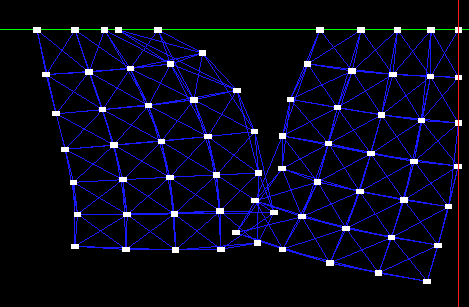
\includegraphics[height=4cm]{img/curtain2.png}
  \captionof{figure}{Two cloth curtains colliding}
  \label{fig:flag2}
\end{minipage}
\end{figure}




\section{Conclusion}

We started with the implementation of a global system to solve all forces and constraints.
With these forces and constraints we made some nice scenes such as hair and cloth, as shown in the results.
The user can also apply forces by interacting with the mouse.
Because the euler integration method is not very stable other integration methods where implemented.
Finally collision detection is implemented such as particle collisions and fixed object collisions.

\end{document}
